\documentclass{report}

\input{~/dev/latex/template/preamble.tex}
\input{~/dev/latex/template/macros.tex}

\title{\Huge{Calculus 1 Notes}}
\author{\huge{Nathan Warner}}
\date{\huge{December 17, 2023}}
\graphicspath{{./images}}

\begin{document}
    \maketitle

    \begin{center}
        \Huge{Chapter 2}
    \end{center}
    \line(1,0){470} 

    \bigbreak \noindent \bigbreak \noindent  
    \begin{Huge}
        \noindent \textbf{Contents}
    \end{Huge}
    
    \bigbreak \noindent \bigbreak \noindent 
    \begin{Large}
        \textbf{2.1: The Tangent and Velocity Problems }
        \bigbreak \noindent \bigbreak \noindent  
        \textbf{2.2.1 The Limits of a Function }
        \bigbreak \noindent \bigbreak \noindent  
        \textbf{2.2.2 Infinite Limits }
        \bigbreak \noindent \bigbreak \noindent 
        \textbf{2.2.3 Finding Limits of a Trigonometric Function }
        \bigbreak \noindent \bigbreak \noindent 
        \textbf{2.3 Calculating Limits Using Limit Laws}
        \bigbreak \noindent \bigbreak \noindent 
        \textbf{2.5.1 Continuity }
        \bigbreak \noindent \bigbreak \noindent 
        \textbf{2.5.2 One-Sided Continuity}
        \bigbreak \noindent \bigbreak \noindent 
        \textbf{2.6 Limits at Infinity: Horizontal Asymptotes}
        \bigbreak \noindent \bigbreak \noindent  
        \textbf{2.7 Derivatives and Rates of Change}
        \bigbreak \noindent \bigbreak \noindent 
        \textbf{2.8.1 The Derivative of a Function}
        \bigbreak \noindent \bigbreak \noindent 
        \textbf{2.8.2 Finding The Derivatives Using The Limit Definition}
    \end{Large}

    \pagebreak
    \begin{Large}
        \noindent \textbf{2.1: The Tangent and Velocity Problems}
    \end{Large}

    \bigbreak \noindent \bigbreak \noindent \bigbreak \noindent 
    \begin{large}
       \noindent \textbf{The Tangent Problem: } 
    \end{large}
   
    \bigbreak \noindent 
    \qs{}{Can we find an equation of the tangent line to $y=x^2$ at the point P(1,1)?}
   
    \bigbreak \noindent 
    \begin{center}
        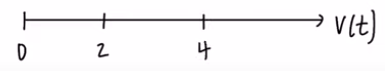
\includegraphics[scale=0.8]{1.png}    
    \end{center}
    
    \pf{Explanation}{. \\
        $y=x^2$: Red parabola \\
        Tangent line: Blue line \\ 
        Secent Line: Pink line with points q and p
    }

    We are asked to get the equation of the tangent line to $y=x^2$ at the point P(1,1), 
    However to find the equation of this line we know we need \textbf{2 things,} 
    \begin{itemize}
        \item Point
        \item Slope
    \end{itemize}

    \noindent Since we only have one point, we cannot find slope. Therefore, we must use 
    another point as an approximation and create a secent line instead. \textbf{This secent line is 
    the pink line in the above graphic.}
    
    \bigbreak \noindent 
    \textbf{So}, lets use the point Q(0,0) as our second point. Now we can find slope with 
    P(1,1), and Q(0,0).

    \bigbreak \noindent 
    \begin{large}
        \textbf{If} Slope = $\frac{y2-y1}{x2-x1}$, Then M of PQ $\rightarrow$ $ \frac{1-0}{1-0}$ = 1
    \end{large}

    \bigbreak \noindent 
    \textbf{Lets} get a better approximation by using a point closer to the tangent line
    Lets use Q(0.9, 0.81)

    \bigbreak \noindent 
    \begin{large}
        \textbf{So} M of PQ $\rightarrow$ $\frac{1-0.81}{1-0.9}$ = 1.9
    \end{large}

    \bigbreak \noindent 
    \textbf{Now}, lets get an even closer approximation by using the point Q(0.99, 0.9801)
    
    \bigbreak \noindent 
    \begin{large}
       \textbf{So}, M of  PQ $\rightarrow$ $ \frac{1-0.9801}{1-0.99}$ = 1.99
    \end{large}

    \pagebreak
    \noindent \textbf{Notice}, as the point Q gets closer to P, the slope of PQ is getting closer to 2
    
    \bigbreak \noindent 
    \textbf{We write}, 
    \begin{center}
        \begin{large}
            $\lim\limits_{Q \to P}${M of PQ} = m
        \end{large}
    \end{center}

    \bigbreak \noindent 
    Where \textbf{m} on the right of equation is slope of tangent line at \textbf{P}, 
    And \textbf{M of PQ} is slope of the secent line

    \bigbreak \noindent \bigbreak \noindent 
    \begin{large}
        \textbf{Now,}     
    \end{large}
    \bigbreak \noindent 
    We will use our approximation of $m \approx 2$ to write the equation of the tangent line,
    using the orginial point P(1,1).

    \begin{align*}
        y-1=2\left(x-1\right) \\
        y-1=2x-2 \\
        y=2x-1
    .\end{align*}
    
    
    \pagebreak
    \begin{large}
       \noindent \textbf{The Velocity Problem:} 
    \end{large}
    
    \bigbreak \noindent \bigbreak \noindent 
    \begin{itemize}
        \item Average Velocity: $\frac{distance\ traveled}{time\ elapsed}$, which is 
            represented by the slope of the secent line.
        \item Instantaneous Velocity = Velocity at a given instant of time, which is represented 
            by the slope of the tangent line
    \end{itemize}

    \bigbreak \noindent \bigbreak \noindent  
    \ex{}{If a rock is thrown upward on the planet Mars, with a Velocity of 10 m/s, It's
    height in meters t seconds later is  given by $y=10t-1.86t^2$}

    \bigbreak \noindent 
    \qs{}{Find the average Velocity over the given time intervals:}
    
    \bigbreak \noindent 
    \textbf{(i)} \textbf{[1,2]} $\rightarrow$ 1 and 2 represent values of \textit{t}
    
    \bigbreak \noindent 
    \begin{center}
        Substitute values into equation above
    \end{center}
    \begin{align*}
        y\left(1\right)=10\left(1\right)-1.86\left(1\right)^2 \\
        = 8.14
    .\end{align*}

    \begin{align*}
        y\left(2\right)=10 \left(2\right) - 1.86 \left(2\right) ^2 \\
        = 12.56
    .\end{align*}

    \bigbreak \noindent 
    \textbf{If} Average Velocity = $\frac{distance\ traveled}{time\ elapsed}$ Or better yet
    $ \frac{Change\ in\ height}{change\ in\ time}$

    \bigbreak \noindent 
    \textbf{And} we have the points (1,8.14) and (2,12.56)

    \bigbreak \noindent 
    \textbf{Then,}

    \begin{align*}
        Average\ Velocity = \frac{12.56-8.14}{2-1} \\
        =4.42 m\diagdown s
   .\end{align*}

    \pagebreak
    \textbf{(ii) [1,1.5]}
    
    \begin{center}
        Substitute values into equation above
    \end{center}
    \begin{align*}
        y\left(1\right)=10\left(1\right)-1.86\left(1\right)^2 \\
        = 8.14
    .\end{align*}

    \bigbreak \noindent 
    \begin{align*}
        y \left(1.5\right) = 10 \left(1.5\right) - 1.86 \left(1.5\right) ^2 \\
        =10.815 
    .\end{align*}

    \bigbreak \noindent 
    \textbf{After} solving theses equations we have the points (1,8.14) and (1.5,10.815)
    \bigbreak \noindent 
    \textbf{So,}
    
    \begin{align*}
        Average\ Velocity = \frac{10.815-8.14}{1.5-1} \\
        = 5.35 m \diagdown s
    .\end{align*}


    \pagebreak
    \begin{Large}
        \textbf{2.1.1 The Limit of a Function:}
    \end{Large}
    
   \bigbreak \noindent \bigbreak \noindent  
    \qs{}{Consider the values of $f \left(x\right) = x^2$ + 2 near $x=2$}

    \bigbreak \noindent 
    We want to know whats going on near x=2, so we make a table

    \bigbreak \noindent 
    \begin{center}
        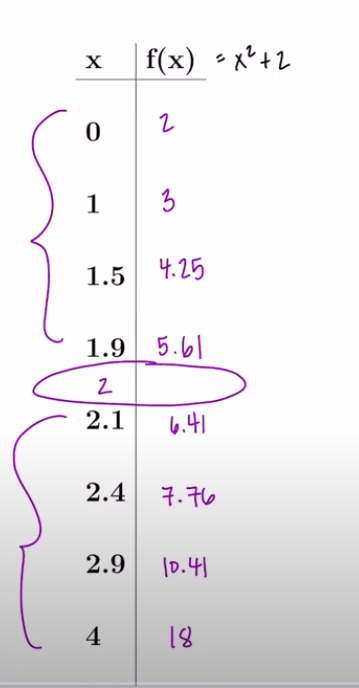
\includegraphics[scale=0.5]{./images/tbale.png}
    \end{center}

    \textbf{Now} we want to look at the closet x values to 2, 
    which is the 2 that are above and below \textbf{2}, \textbf{We observe that as x values approach
    2, then f(x) values approach 6}

    \bigbreak \noindent 
    \textbf{so we write,}    

    \begin{large}
        \begin{align*}
            \lim\limits_{x \to 2}{f \left(x\right) = 6}
        .\end{align*}
    \end{large}
    
    \bigbreak \noindent 
    \ex{}{Use a table of values to estimate the limit:$\lim\limits_{x \to 0 }{ \frac{tan3x}{tan5x}}$}
    
    \bigbreak \noindent 
    Rememeber the value \textbf{0} is \textbf{a} so we want to contruct our table where a 
    is in the middle, so use values that are smaller and larger than a.

    \bigbreak \noindent 
    Using arbitrary values that are close to 0, we gete the table, 

    \bigbreak \noindent 
    \begin{center}
        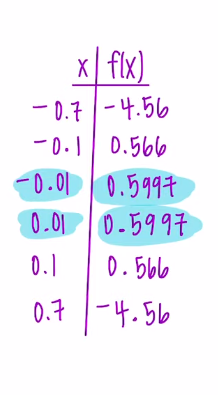
\includegraphics[scale=0.5]{./images/table2.png}
    \end{center}
    
    \bigbreak \noindent 
    Now after looking at our table, we can conclude that

    \bigbreak \noindent 

    \begin{large}
        \begin{align*}
            \lim\limits_{x \to0 }{ \frac{tan3x}{tan5x} = 0.6}
        .\end{align*}
    \end{large}

    \pagebreak
    \begin{large}
        \noindent \textbf{One Sided Limits:}
    \end{large}
   
    
    \bigbreak \noindent 
    \begin{center}
        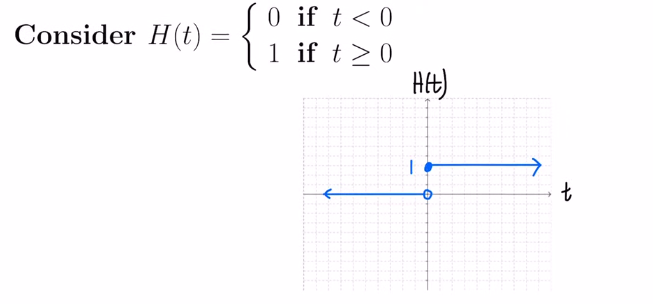
\includegraphics[scale=0.5]{./images/ht.png} 
    \end{center}

    \bigbreak \noindent \bigbreak \noindent 
    \nt{if there is a \textbf{minus} sign after a, that means you are approaching limit from the left
        if there is a \textbf{plus} sign after a, that means you are approaching limit from the right, 
        if you see a limit with either of these, it is called a two sided limit
    }
    \bigbreak \noindent 
    \textbf{What is $\lim\limits_{t \to 0- }{h \left(t\right)}$}

    \bigbreak \noindent 
    So looking at the bottom line, coming from the left, as we approach 0, the y value is 
    0.

    \bigbreak \noindent 
    \textbf{so $\rightarrow$}

    \begin{align*}
        \lim\limits_{t \to 0- }{h \left(t\right) = 0}
    .\end{align*}


    \bigbreak \noindent 
    \textbf{What is $\lim\limits_{t \to 0+}{h \left(t\right)}$} 

    \bigbreak \noindent 
    Given that we are approaching from the right, we are now looking at the top line, 
    we can see that as we approach 0, y is 1

    \bigbreak \noindent 
    \textbf{so}

    \begin{align*}
        \lim\limits_{t \to 0+ }{h \left(t\right) = 1}
    .\end{align*}

    \bigbreak \noindent 
    \nt{The first one is our \textbf{Left hand limit} and the bottom one is our \textbf{right hand limit} 
        if the side we our approaching from is not specified, \textbf{we cannot find the limit, so we would say DNE}
    }

    \bigbreak \noindent 
    \textbf{So}

    \bigbreak \noindent 
    $\lim\limits_{x \to 0}{f \left(x\right) = l}$ \textbf{iff} (if and only if) $\lim\limits_{x \to 0- }{f \left(x\right) = L}$ \textbf{and} $\lim\limits_{x \to 0+ }{f \left(x\right) = L}$

    \bigbreak \noindent 
    in other words, we can only drop the + or - after the a if the right and left hand limits are the same

    \pagebreak
    \begin{large}
       \noindent \textbf{Infinite Limits:} 
    \end{large}
    
    \bigbreak \noindent \bigbreak 
    \begin{center}
        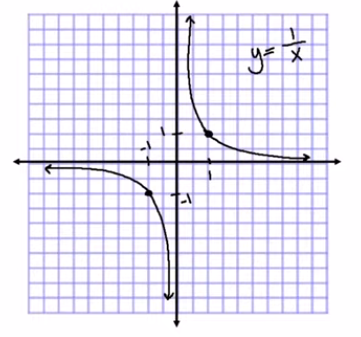
\includegraphics[scale=0.7]{./images/graph.png}
    \end{center}
    
    \bigbreak \noindent 
    \textbf{if we look at }

    \begin{large}
        \begin{align*}
            \lim\limits_{x \to 0+}{f(x) = ?}
        .\end{align*}
    \end{large}
    
    \bigbreak \noindent 
    We notice that as we approach 0 from the right, f(x) goes to infinity

    \bigbreak \noindent 
    \textbf{So:}
    
    \begin{large}
        \begin{align*}
            \lim\limits_{x \to 0+}{f(x) = \infty}
        .\end{align*}
    \end{large}
    
    \bigbreak \noindent 
    This is also the same for x $\rightarrow$ $0-$
    
    \bigbreak \noindent 
    \textbf{So:}

    \begin{large}
        \begin{align*}
            \lim\limits_{x \to 0-}{f \left(x\right) = \infty}
        .\end{align*}
    \end{large}

    \bigbreak \noindent 
    \nt{x = 0 is a vertical Asymptote}

    \begin{center}
        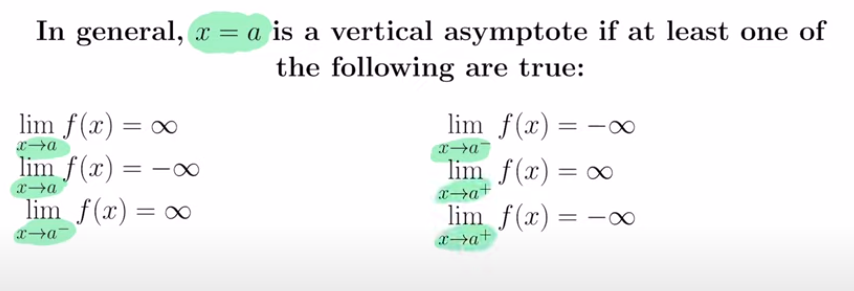
\includegraphics[scale=0.5]{./images/ass.png}
    \end{center}

    \bigbreak \noindent \bigbreak \noindent 
    \begin{large}
       \textbf{Examples: Determine the infitite limit} 
    \end{large}

    \bigbreak \noindent 
    \begin{large}
       \textbf{1.)} $\lim\limits_{x \to 5-}{ \frac{x+1}{x-5}}$ 
    \end{large}
    
    \bigbreak \noindent \bigbreak \noindent 
    \begin{center}
        \begin{large}
            x + 1 $\longrightarrow$ 6 \\
            x - 5 $\longrightarrow$ 0 
        \end{large}
    \end{center}

    \bigbreak 
    \begin{large}
        If you have a $ \frac{nonzero\ constant}{approaching\ 0} $ 
        its either going to be approaching $\infty$ or $-\infty$ the way we find which version of infinity
        it will be is with either a table or a numberline
    \end{large}
    
    \bigbreak 
    To make the numerline we want to list the zeros, so -1 and 5. Then pick a value thats close to a
    and approachs in the correct direction. Then plug this number into the equation and whatever sign you get
    will be the sign for infinity.
    \bigbreak \noindent 
    \begin{center}
        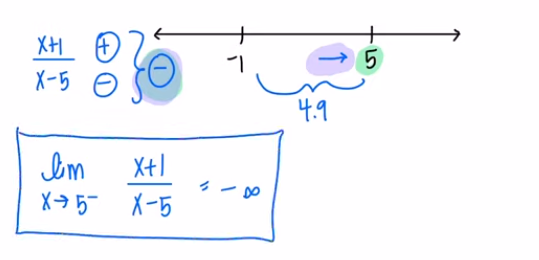
\includegraphics[scale=.5]{./images/line.png}
    \end{center}
    
    \bigbreak \noindent \bigbreak \noindent  
    \begin{large}
        \textbf{2.)} $\lim\limits_{x \to 5-}{ \frac{e^x}{ \left(x-5\right)^3}}$ 
    \end{large}

    \bigbreak \noindent 
    \begin{center}
       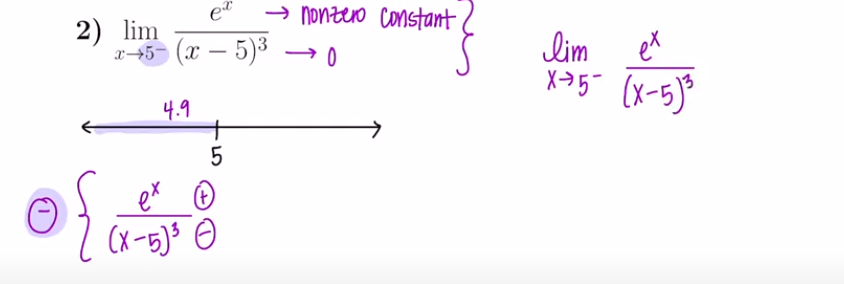
\includegraphics[scale=0.5]{ ./images/abc.png } 
    \end{center}
    
    
    
    


\end{document}
